%%%%%%%%%%%%%%%%%%%%%%%%%%%%%%%%%%%%%%%%%
% University/School Laboratory Report
% LaTeX Template
% Version 3.0 (4/2/13)
%
% This template has been downloaded from:
% http://www.LaTeXTemplates.com
%
% Original author:
% Linux and Unix Users Group at Virginia Tech Wiki 
% (https://vtluug.org/wiki/Example_LaTeX_chem_lab_report)
%
% License:
% CC BY-NC-SA 3.0 (http://creativecommons.org/licenses/by-nc-sa/3.0/)
%
%%%%%%%%%%%%%%%%%%%%%%%%%%%%%%%%%%%%%%%%%

%----------------------------------------------------------------------------------------
%	PACKAGES AND DOCUMENT CONFIGURATIONS
%----------------------------------------------------------------------------------------

\documentclass{article}

\usepackage[version=3]{mhchem} % Package for chemical equation typesetting
\usepackage{siunitx} % Provides the \SI{}{} command for typesetting SI units

\usepackage{graphicx}
\usepackage{caption}
\usepackage{subcaption}
\usepackage{cancel}

\usepackage{float}

\usepackage[T1]{fontenc} % allow small bold caps

\usepackage{listings}
\usepackage{color}

\definecolor{dkgreen}{rgb}{0,0.6,0}
\definecolor{gray}{rgb}{0.5,0.5,0.5}
\definecolor{mauve}{rgb}{0.58,0,0.82}

\lstset{frame=tb,
  language=Matlab,
  aboveskip=2mm,
  belowskip=2mm,
  showstringspaces=false,
  columns=flexible,
  basicstyle={\small\ttfamily},
  numbers=none,
  numberstyle=\tiny\color{gray},
  keywordstyle=\color{blue},
  commentstyle=\color{dkgreen},
  stringstyle=\color{mauve},
  breaklines=true,
  breakatwhitespace=true
  tabsize=2
}

\setlength\parindent{0pt} % Removes all indentation from paragraphs

\renewcommand{\labelenumi}{\alph{enumi}.} % Make numbering in the enumerate environment by letter rather than number (e.g. section 6)

\usepackage[margin=1in]{geometry}

\usepackage{amssymb}


%\usepackage{times} % Uncomment to use the Times New Roman font

%----------------------------------------------------------------------------------------
%	Title
%----------------------------------------------------------------------------------------

\begin{document}
\pagenumbering{gobble}

\title{6.s02: EECS II - From A Medical Perspective}
\author{
  Ryan Lacey <rlacey@mit.edu>\\
  \footnotesize \texttt{Collaborator(s): Daniel Moon}
}
        
\maketitle
        

\begin{enumerate}
\item[1.]
	\begin{enumerate}
	\item[(a)]
	$M_{xy}(t) = M_{xy}(0)e^{-t/T_2}$\\
	$\therefore M_{xyA}(t) = M_{xy}(0)e^{-t/T_2A}$\\
	
	$M_z(t) = M_0 + (M_z(0) - M_0)e^{-t/T_1}$\\
	No component of field in longitudinal direction after  excitation.\\
	$\therefore M_{zA}(t) = M_0 - M_0 e^{-t/T_{1A}}$\\

	\item[(b)]
\begin{align*}
|\Delta S_{xy}(t)| &= |M_{xyA}(t) - M_{xyB}(t)|\\
&= M_{0} e^{-t/T_{2A}} - M_{0} e^{-t/T_{2B}}\\
\text{Maximize}&\\
0 &= \frac{d}{dt} M_{0} \left(e^{-t/T_{2A}} - e^{-t/T_{2B}} \right)\\
t &= \left( \frac{1}{T_{2A}} - \frac{1}{T_{2B}} \right)^{-1} \ln \left( \frac{T_{2B}}{T_{2A}} \right)
\end{align*}

	\item[(c)]
\begin{align*}
|\Delta S_{z}(t)| &= |M_{zA}(t) - M_{zB}(t)|\\
&= \left(M_0 - M_0 e^{-t/T_{1A}} \right) - \left( M_0 - M_0 e^{-t/T_{1B}} \right)\\
\text{Maximize}&\\
t &= \left( \frac{1}{T_{1A}} - \frac{1}{T_{1B}} \right)^{-1} \ln \left( \frac{T_{1B}}{T_{1A}} \right)
\end{align*}

	\item[(d)]
	Transverse: $\left( \frac{1}{92} - \frac{1}{100} \right)^{-1} \ln \left( \frac{100}{92} \right) = 95.88s$\\
	Longitudinal: $\left( \frac{1}{680} - \frac{1}{810} \right)^{-1} \ln \left( \frac{810}{680} \right) = 741.21s$
	\end{enumerate}

\newpage

\item[2.]
	\begin{enumerate}
	\item[(a)] $\;$\\
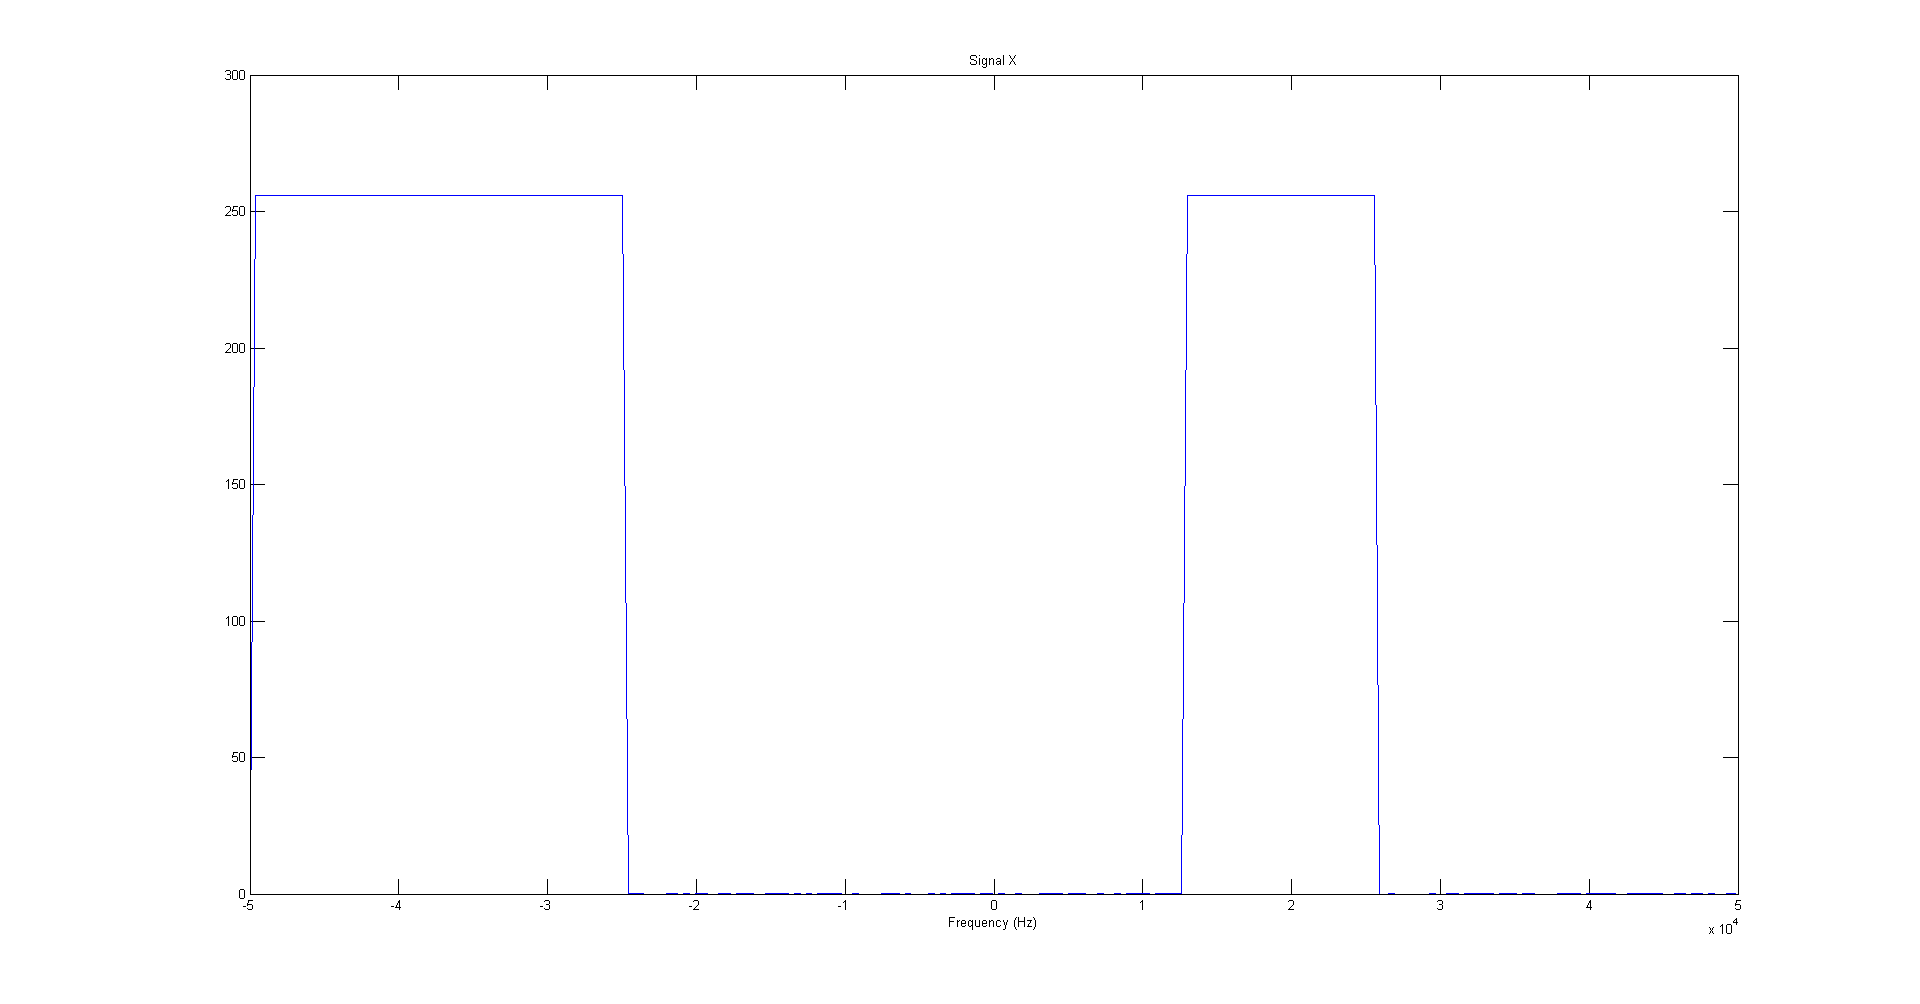
\includegraphics[width=\textwidth]{../images/SignalX} \\
	\item[(b)] $\;$\\
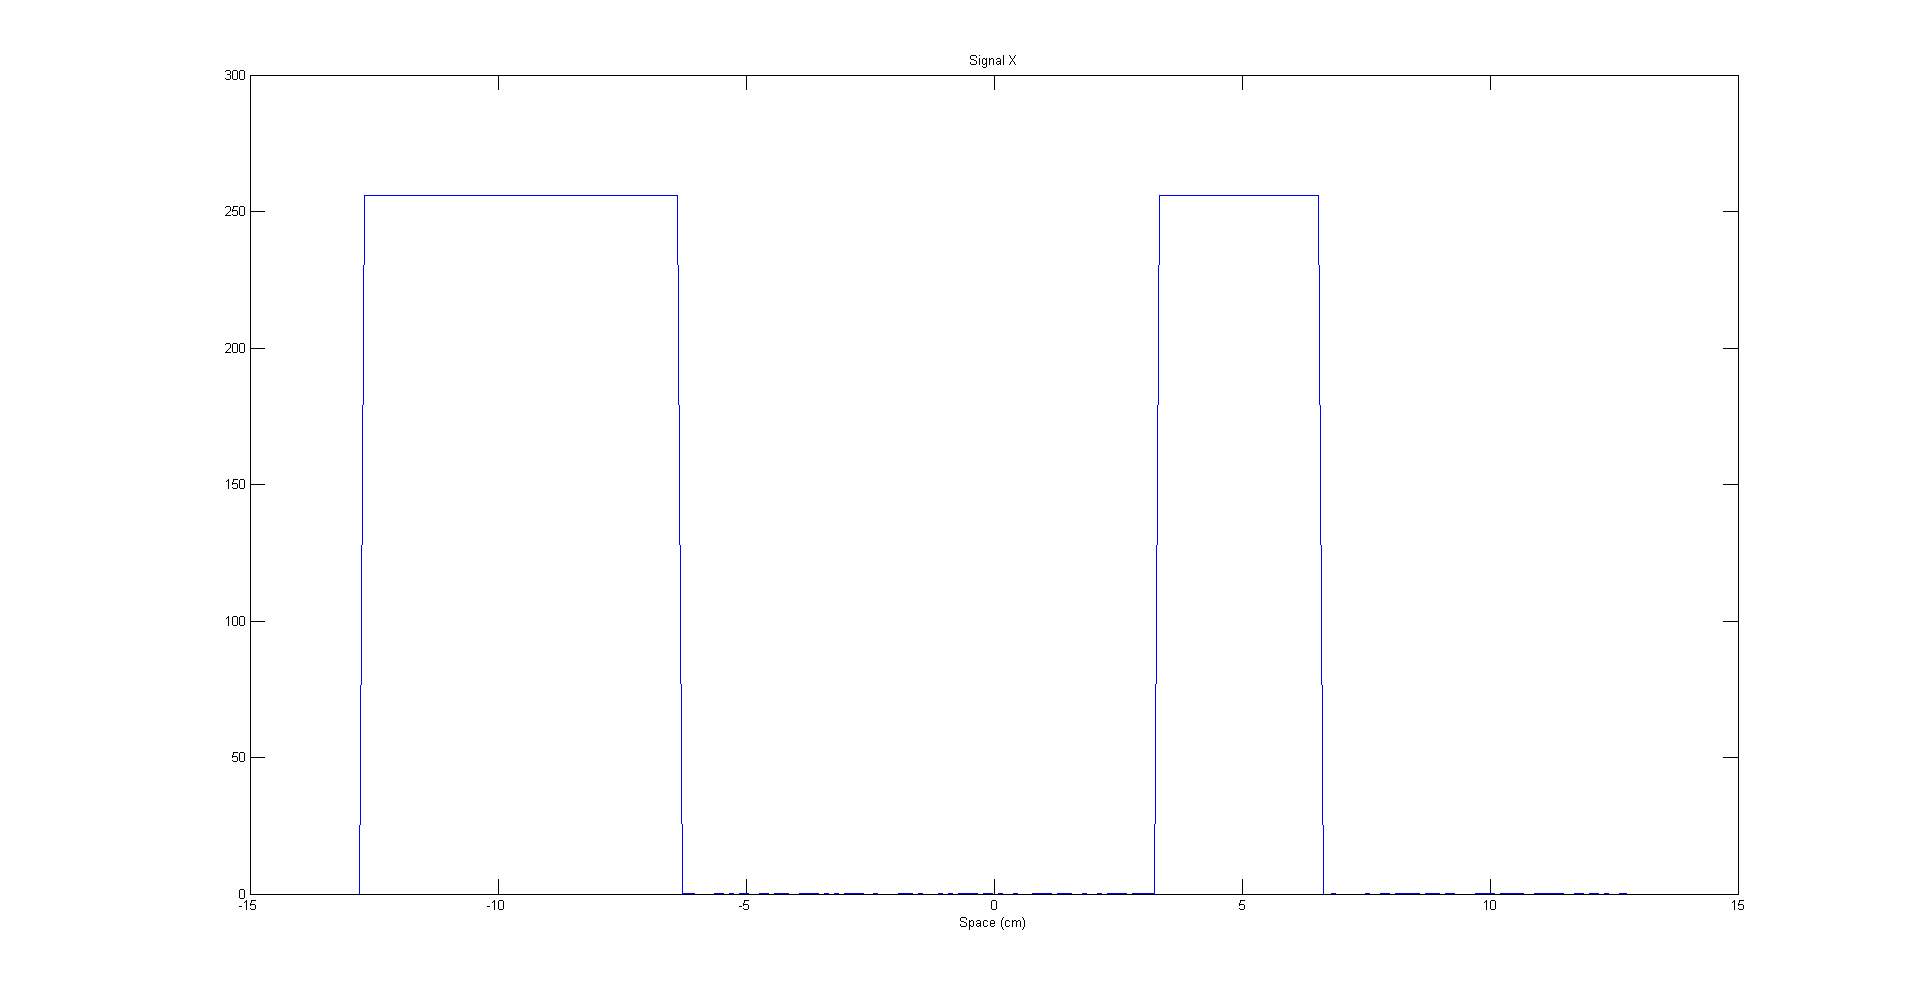
\includegraphics[width=\textwidth]{../images/SpaceX} \\

\newpage

	\item[(c)] $\;$\\
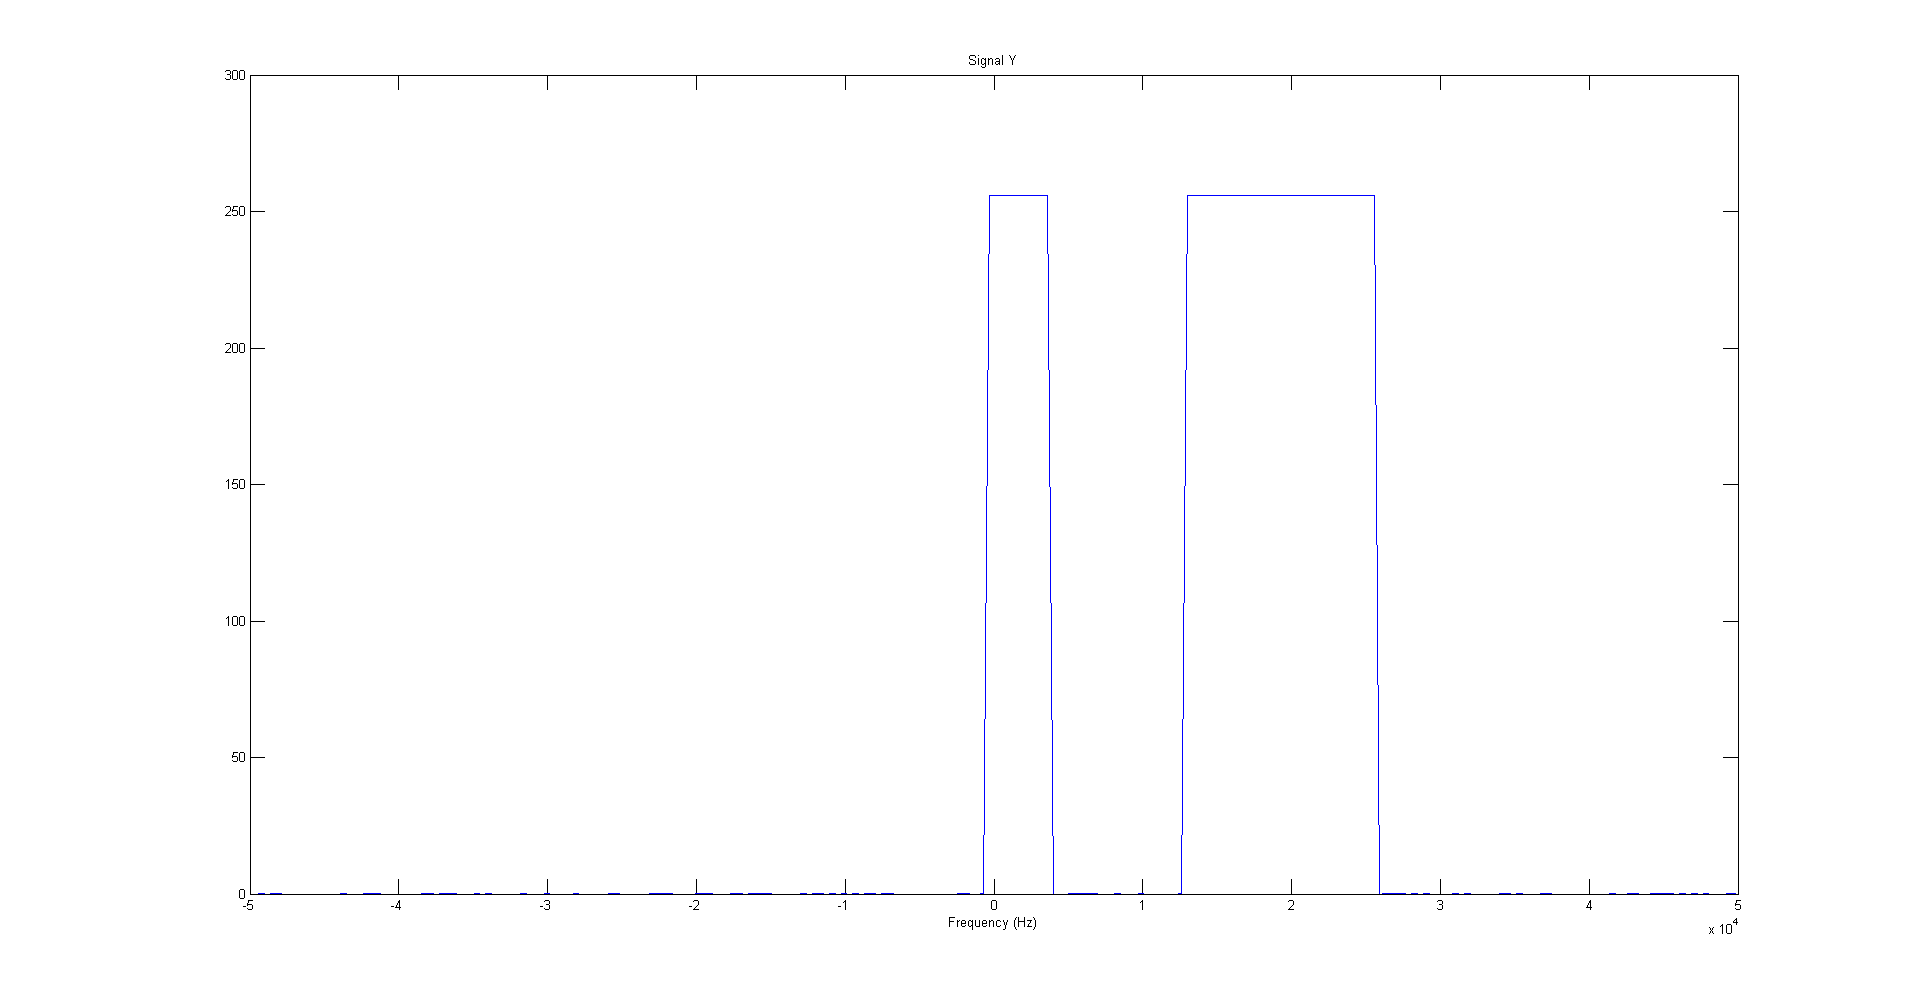
\includegraphics[width=\textwidth]{../images/SignalY} \\
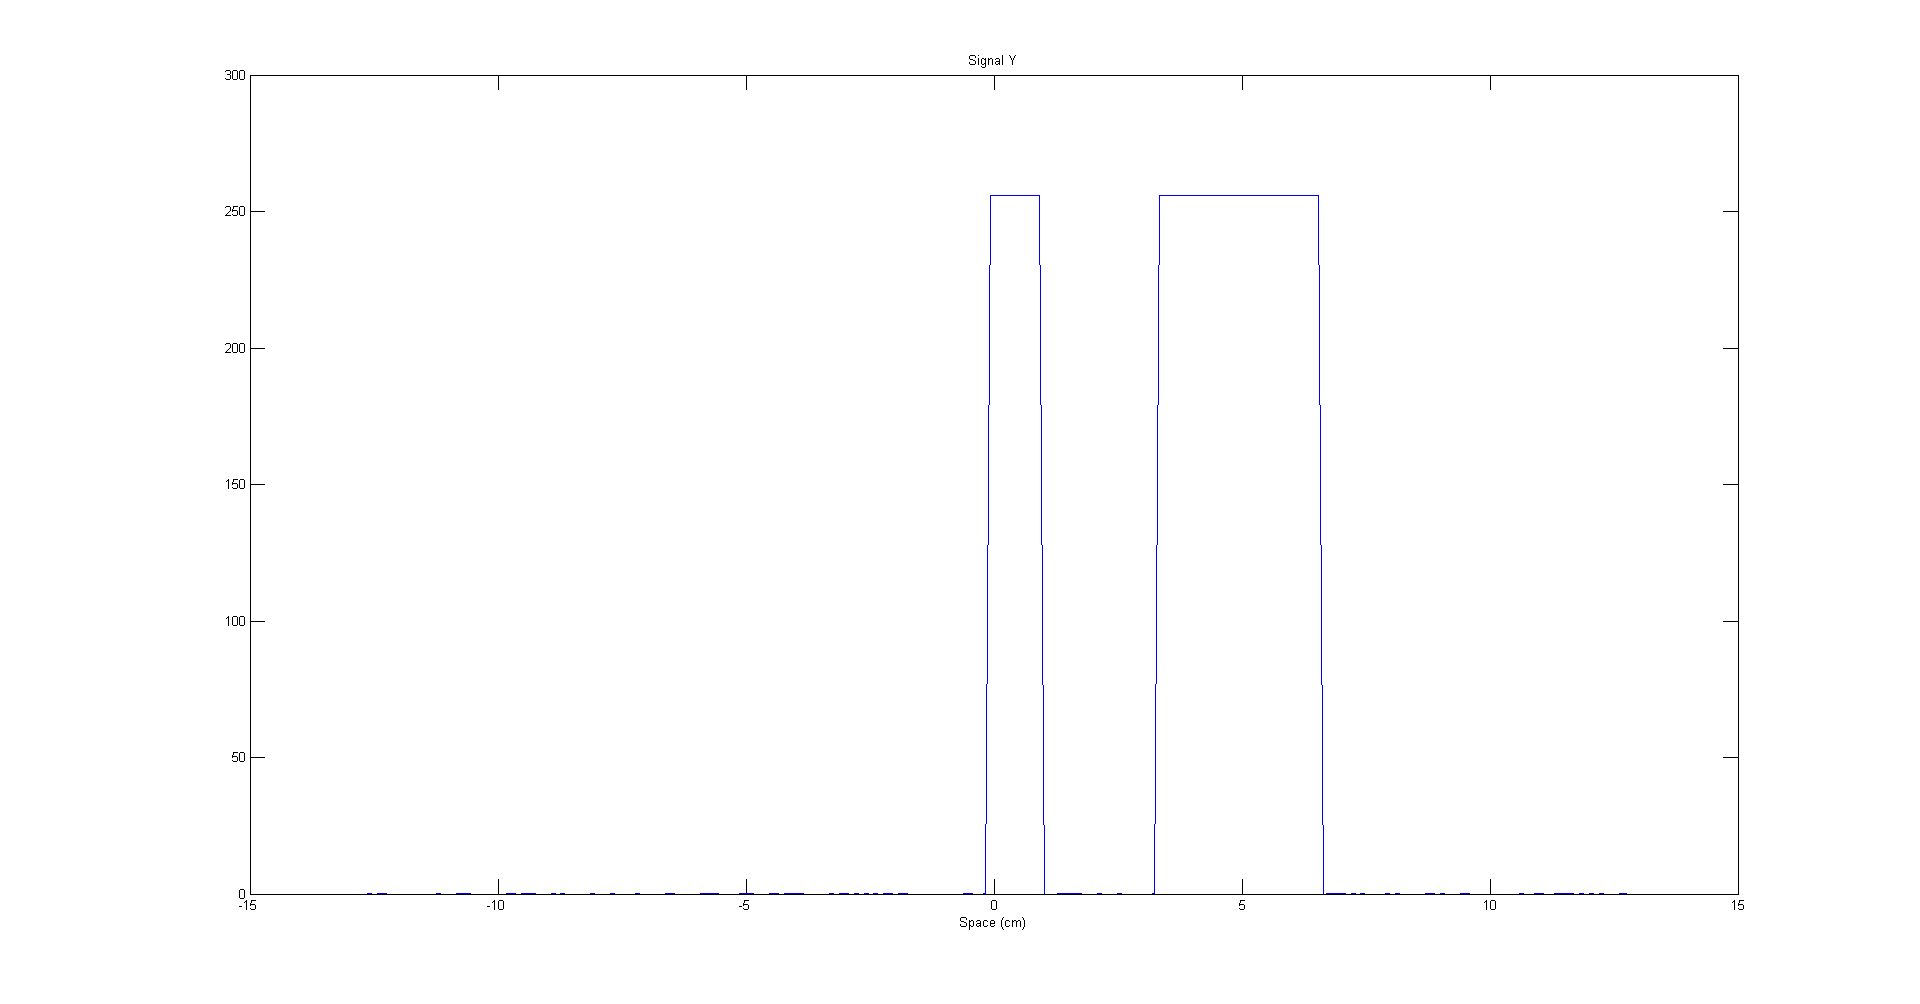
\includegraphics[width=\textwidth]{../images/SpaceY} \\

\newpage 

\begin{lstlisting}   
f = linspace(-50000, 100000*(1-1/256)/2, 256);
xfft = fftshift(fft(signal_x));
yfft = fftshift(fft(signal_y));
gamma = 42577;
G = 9.176;
dist = f*100 / (G*gamma);
% Frequency X
plot(f, abs(xfft))
xlabel('Frequency (Hz)')
title('Signal X')
% Frequency Y
plot(f, abs(yfft))
xlabel('Frequency (Hz)')
title('Signal Y')
% Space X
plot(dist, abs(xfft))
xlabel('Space (cm)')
title('Signal X')
% Space Y
plot(dist, abs(yfft))
xlabel('Space (cm)')
title('Signal Y')
\end{lstlisting}
	\end{enumerate}
\end{enumerate}

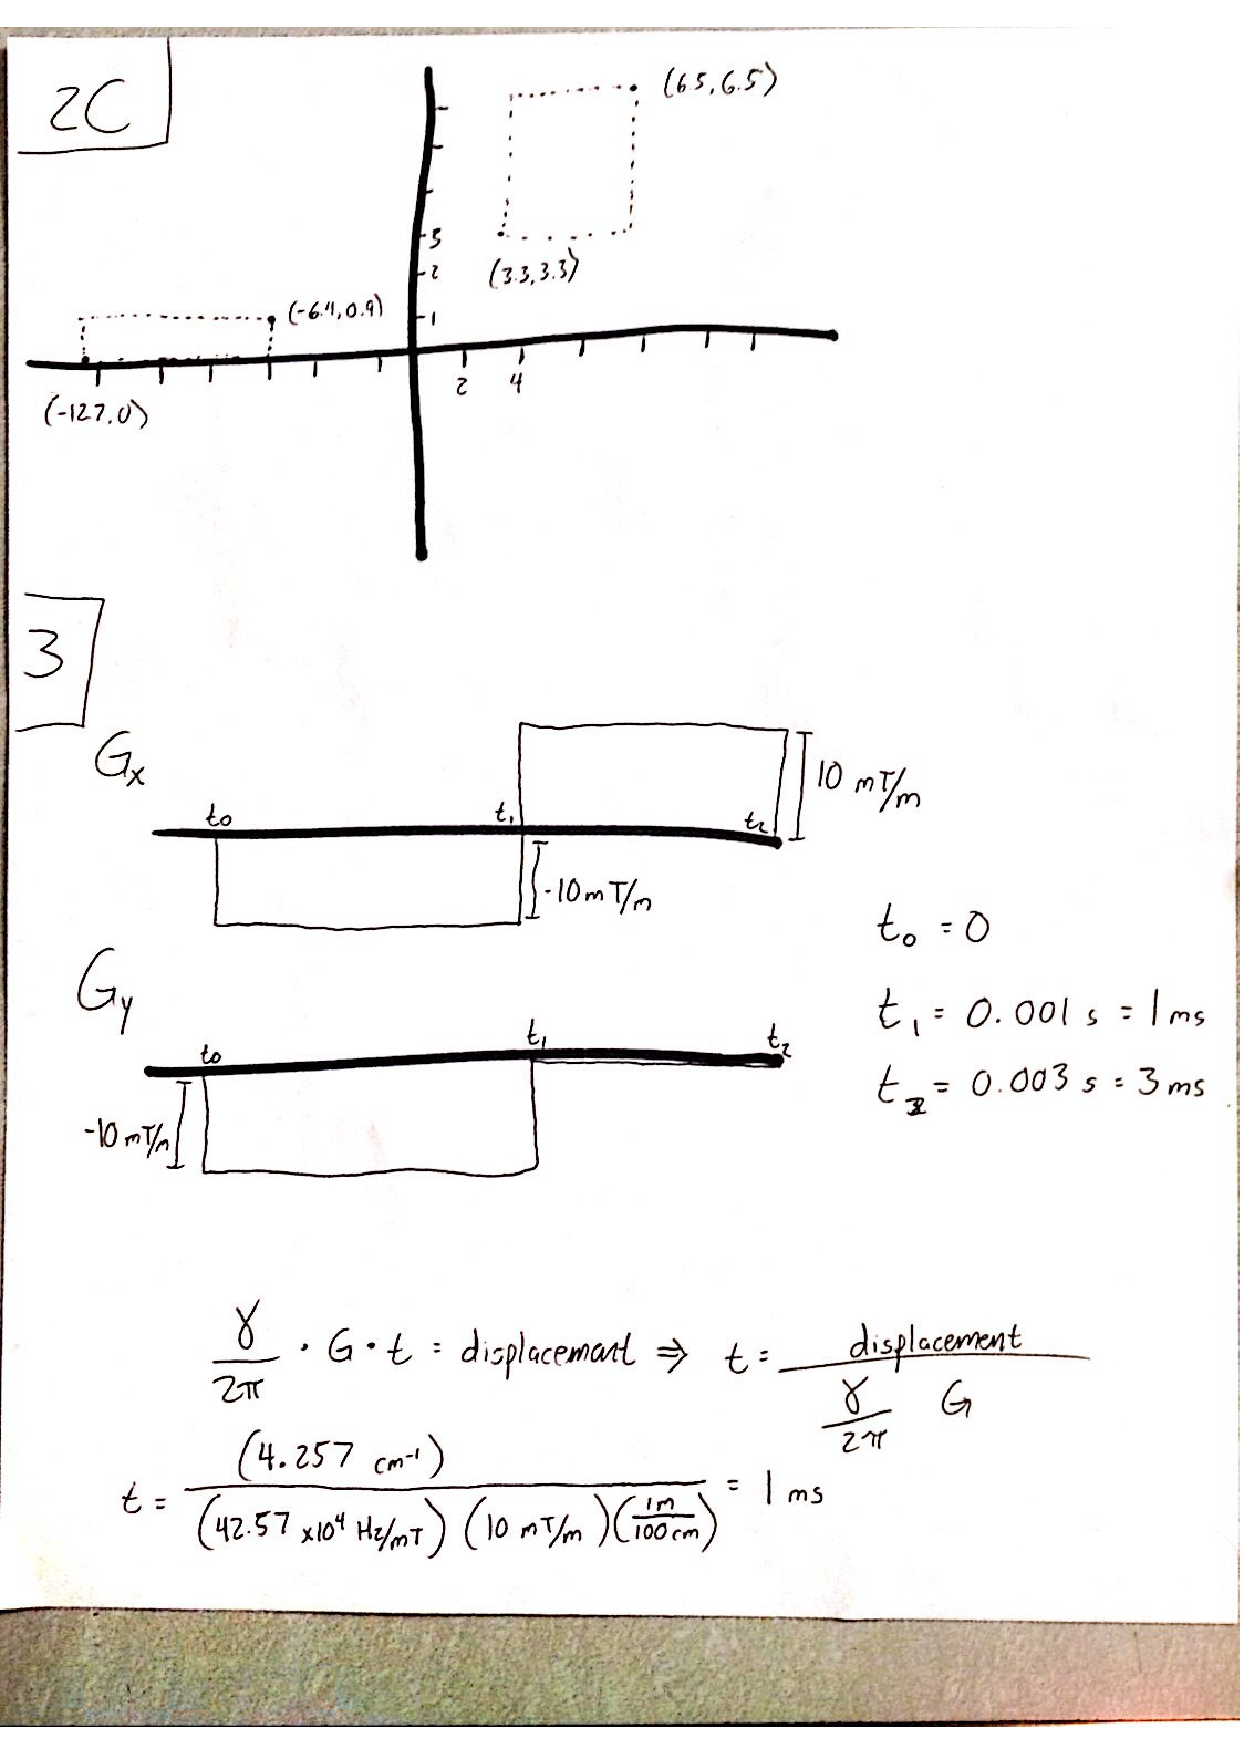
\includegraphics[width=\textwidth]{../images/Problems2&3} \\

\end{document}